\documentclass[11pt,a4paper]{article}

\usepackage[utf8]{inputenc}
\usepackage[T1]{fontenc}
\usepackage{geometry}
\geometry{margin=2.5cm}
\usepackage{graphicx}
\usepackage{amsmath,amssymb}
\usepackage{booktabs}
\usepackage{hyperref}
\usepackage{listings}
\usepackage{xcolor}
\usepackage{caption}
\usepackage{float}

\lstset{
  language=Python,
  basicstyle=\ttfamily\footnotesize,
  keywordstyle=\color{blue},
  commentstyle=\color{gray},
  stringstyle=\color{red!70!black},
  numbers=left,
  numberstyle=\tiny\color{gray},
  frame=single,
  breaklines=true,
  showstringspaces=false,
  tabsize=4,
  extendedchars=true,
  inputencoding=utf8,
  literate=
    {×}{{$\times$}}1
    {≈}{{$\approx$}}1
    {—}{{---}}1
    {→}{{$\rightarrow$}}1
    {λ}{{$\lambda$}}1
    {α}{{$\alpha$}}1
}

\title{Fast Matrix Factorization for Online Recommendation\\with Implicit Feedback\\[0.5em]\large Data Management Project Report}
\author{[Student Names]\\
  \'Ecole Polytechnique}
\date{April 2026}

\begin{document}
\maketitle

% ============================================================
\section{Description of the Adopted Solution}
% ============================================================

\subsection{Problem Setting}

Recommendation systems built on implicit feedback face a different problem than those built on explicit ratings. When a user rates a movie four stars, the signal is direct. When a user watches a movie, all we know is that some interaction occurred. The absence of an interaction is ambiguous: the user may dislike the item, or may simply not know it exists. This asymmetry between observed positives and unobserved (not necessarily negative) entries is the central difficulty.

Hu et al.~\cite{hu2008} formalized this by treating all user-item pairs as data points, assigning a confidence weight $c_{ui}$ to each. Observed interactions receive high confidence ($c_{ui} = 1 + \alpha$), while missing entries receive a low uniform weight $c_0$. The model then minimizes:

\begin{equation}
\mathcal{L} = \sum_{u}\sum_{i} c_{ui}\left(r_{ui} - \mathbf{p}_u^\top \mathbf{q}_i\right)^2 + \lambda\left(\|\mathbf{P}\|^2 + \|\mathbf{Q}\|^2\right)
\label{eq:loss}
\end{equation}

where $r_{ui} = 1$ for observed interactions and $0$ otherwise, $\mathbf{P} \in \mathbb{R}^{M \times k}$ and $\mathbf{Q} \in \mathbb{R}^{N \times k}$ are the user and item latent factor matrices, and $\lambda$ controls regularization.

The sum in Equation~\ref{eq:loss} runs over all $M \times N$ pairs, including the enormous number of zeros. Standard ALS solves this by alternating between fixing $\mathbf{Q}$ and solving for each $\mathbf{p}_u$ (and vice versa), but each user update requires constructing and inverting a $k \times k$ matrix that depends on all $N$ items. The per-user cost is $O(Nk^2)$, which becomes prohibitive for large item catalogs.

\subsection{The eALS Algorithm}

He et al.~\cite{he2016} proposed element-wise ALS (eALS), which restructures the update to avoid iterating over all items. Instead of solving a $k$-dimensional linear system per user, eALS updates one latent factor at a time. The trick is to precompute:

\begin{equation}
\mathbf{S}^q = \mathbf{Q}^\top \mathbf{Q} \in \mathbb{R}^{k \times k}
\end{equation}

This small matrix captures the aggregate contribution of all items. With $\mathbf{S}^q$ in hand, the closed-form update for user $u$, factor $f$ becomes:

\begin{equation}
p_{uf} = \frac{\displaystyle\sum_{i \in \mathcal{I}_u} (c_{ui} - c_0)\, q_{if}\, \hat{r}_{ui}^{(f)} \;-\; c_0\left(\mathbf{p}_u^\top \mathbf{S}^q_{:,f} - p_{uf}\, S^q_{ff}\right)}{\displaystyle\sum_{i \in \mathcal{I}_u} (c_{ui} - c_0)\, q_{if}^2 \;+\; c_0\, S^q_{ff} \;+\; \lambda}
\label{eq:update}
\end{equation}

where $\hat{r}_{ui}^{(f)} = 1 - \sum_{f' \neq f} p_{uf'}\, q_{if'}$ is the residual with factor $f$ removed, and $\mathcal{I}_u$ is the set of items user $u$ interacted with. The numerator's first term sums only over observed items ($|\mathcal{I}_u|$ terms). The second term uses $\mathbf{S}^q$ to account for all items without enumerating them. This brings the per-user cost down to $O(|\mathcal{I}_u| \cdot k + k^2)$.

\subsection{Why This Approach}

We chose eALS for two reasons. First, the element-wise update avoids the $O(Nk^2)$ bottleneck of standard ALS, making it practical on larger datasets. Second, the structure is well-suited to distributed computation: when updating user factors, each user's computation depends only on the (broadcast) item matrix $\mathbf{Q}$ and the precomputed $\mathbf{S}^q$, with no dependencies between users. This makes the user-update step embarrassingly parallel, and likewise for the item-update step.

We implemented the algorithm in Python using NumPy (as a reference) and PySpark RDDs (for distributed execution), and evaluated it on the MovieLens 100K dataset using the leave-one-out protocol.


% ============================================================
\section{Algorithm Design}
% ============================================================

\subsection{Overall Structure}

Each iteration of eALS consists of two symmetric half-steps:

\begin{enumerate}
\item \textbf{User update.} Compute $\mathbf{S}^q = \mathbf{Q}^\top \mathbf{Q}$. For each user $u$, update $p_{u0}, p_{u1}, \ldots, p_{u,k-1}$ sequentially using Equation~\ref{eq:update}. After updating $p_{uf}$, refresh a prediction cache so that $\hat{r}_{ui}^{(f+1)}$ can be computed cheaply.

\item \textbf{Item update.} Compute $\mathbf{S}^p = \mathbf{P}^\top \mathbf{P}$. For each item $i$, update $q_{i0}, q_{i1}, \ldots, q_{i,k-1}$ using the symmetric formula (swapping roles of $\mathbf{P}$ and $\mathbf{Q}$).
\end{enumerate}

The prediction cache avoids recomputing $\mathbf{p}_u^\top \mathbf{q}_i$ from scratch after each factor update. When $p_{uf}$ changes by $\delta$, the cache is patched: $\text{cache}[i] \mathrel{+}= \delta \cdot q_{if}$, costing $O(|\mathcal{I}_u|)$ instead of $O(|\mathcal{I}_u| \cdot k)$.

\subsection{Complexity}

Per iteration, the cost breaks down as:
\begin{itemize}
\item Precomputing $\mathbf{S}^q$: $O(Nk^2)$
\item Updating all users: $O\!\left(\sum_u |\mathcal{I}_u| \cdot k + M k^2\right) = O(|\mathcal{R}|\,k + Mk^2)$
\item Precomputing $\mathbf{S}^p$ and updating all items: $O(|\mathcal{R}|\,k + Nk^2)$
\end{itemize}
Total: $O(|\mathcal{R}|\,k + (M+N)k^2)$, where $|\mathcal{R}|$ is the number of observed interactions. Compare this to standard ALS at $O((M+N)Nk^2)$. For MovieLens 100K, $|\mathcal{R}| \approx 100\text{K}$ and $MN \approx 1.6\text{M}$, so eALS is already roughly $16\times$ cheaper per iteration.

\subsection{Spark Parallelization Strategy}

The user-update half-step has no data dependencies between users: each user's update reads from $\mathbf{Q}$ and $\mathbf{S}^q$, which are fixed for the duration of the half-step. We parallelize this in Spark as follows:

\begin{enumerate}
\item The driver computes $\mathbf{S}^q$ ($k \times k$, cheap) and broadcasts both $\mathbf{Q}$ and $\mathbf{S}^q$ to all workers.
\item An RDD of \texttt{(user\_id, item\_indices)} is partitioned across workers. Each worker processes its assigned users independently.
\item Updated user vectors are collected back to the driver.
\end{enumerate}

The item-update step is symmetric: broadcast $\mathbf{P}$ and $\mathbf{S}^p$, partition items, collect updated item vectors.

The only synchronization point is between half-steps: all user updates must finish before item updates begin (and vice versa), because item updates read the new $\mathbf{P}$.

\subsection{Code Commentary}

We now describe the main code fragments. The full code is in Appendix~\ref{sec:code}.

\subsubsection{Data Loading and Preprocessing}

The \texttt{data\_loader.py} module handles the pipeline from raw MovieLens files to sparse matrices ready for training.

\begin{lstlisting}[caption={Binarization and minimum-interaction filtering.}]
def binarize(interactions, threshold=0.0):
    binarized = [
        (u, i, 1.0, ts)
        for u, i, r, ts in interactions
        if r > threshold
    ]
    return binarized

def filter_min_interactions(interactions, min_user=5, min_item=0):
    prev_count = len(interactions) + 1
    while len(interactions) < prev_count:
        prev_count = len(interactions)
        if min_user > 0:
            user_counts = defaultdict(int)
            for u, i, v, ts in interactions:
                user_counts[u] += 1
            interactions = [
                (u, i, v, ts) for u, i, v, ts in interactions
                if user_counts[u] >= min_user
            ]
        # symmetric for items
    return interactions
\end{lstlisting}

All ratings are converted to binary signals (line 3): any observed interaction becomes 1. The filtering loop (lines 9--18) iteratively removes users below the threshold, since removing items can push users below the minimum and vice versa. The loop converges in one or two passes for typical datasets.

The train/test split uses a leave-one-out strategy: for each user, the most recent interaction (by timestamp) goes to the test set, and all earlier interactions form the training set. This matches the evaluation protocol in~\cite{he2016}.

\subsubsection{Element-wise User Update (NumPy)}

\begin{lstlisting}[caption={Core element-wise update for user factors.}]
def _update_users(P, Q, R_csr, Sq, c_obs, c0, reg, M, k):
    for u in range(M):
        item_indices = R_csr[u].indices
        if len(item_indices) == 0:
            continue
        Q_u = Q[item_indices]            # |I_u| x k
        pred_cache = Q_u @ P[u]          # |I_u| predictions

        for f in range(k):
            q_f = Q_u[:, f]
            hat_r = 1.0 - pred_cache + P[u, f] * q_f

            numer = (c_obs - c0) * np.dot(q_f, hat_r)
            numer -= c0 * (P[u] @ Sq[:, f] - P[u, f] * Sq[f, f])

            denom = (c_obs - c0) * np.dot(q_f, q_f) + c0 * Sq[f, f] + reg

            old_val = P[u, f]
            P[u, f] = numer / denom
            pred_cache += (P[u, f] - old_val) * q_f
\end{lstlisting}

Line 7 computes $\mathbf{p}_u^\top \mathbf{q}_i$ for all observed items as a single matrix-vector product. The inner loop (line 9) iterates over factors. Line 11 computes $\hat{r}_{ui}^{(f)}$ by removing factor $f$'s contribution from the cached prediction. Lines 13--14 implement the numerator from Equation~\ref{eq:update}: the first term sums over observed items, and the second uses $\mathbf{S}^q$ for the all-items term. Line 20 patches the cache in $O(|\mathcal{I}_u|)$ rather than recomputing from scratch.

\subsubsection{Spark RDD Parallelization}

\begin{lstlisting}[caption={User update distributed via Spark RDD.}]
# Broadcast Q and S^q to all workers
Q_bc = sc.broadcast(Q)
Sq_bc = sc.broadcast(Sq)
P_bc = sc.broadcast(P)

def update_user_partition(iterator):
    q_local = Q_bc.value
    sq_local = Sq_bc.value
    results = []
    for u, item_indices in iterator:
        p_u = P_bc.value[u].copy()
        Q_u = q_local[item_indices]
        pred_cache = Q_u @ p_u
        for f in range(k):
            # ... same element-wise update as NumPy ...
            pass
        results.append((u, p_u))
    return iter(results)

updated_users = user_rdd.mapPartitions(update_user_partition).collect()
for u, p_u in updated_users:
    P[u] = p_u
\end{lstlisting}

The structure mirrors the NumPy version exactly. The difference is that the outer loop over users (line 10) runs inside a Spark partition, and each partition processes a disjoint subset of users in parallel. Lines 2--4 broadcast the read-only data ($\mathbf{Q}$, $\mathbf{S}^q$, $\mathbf{P}$) once to all workers instead of shipping it per-task. Line 20 collects the updated vectors back to the driver, which writes them into $\mathbf{P}$.

We use \texttt{mapPartitions} rather than \texttt{map} to amortize the overhead of deserializing broadcast variables: each worker deserializes once per partition rather than once per user.

\subsubsection{Loss Computation}

Computing the loss naively requires iterating over all $M \times N$ pairs. We avoid this with a decomposition:

\begin{lstlisting}[caption={Efficient loss computation using the trace trick.}]
def _compute_loss(P, Q, R_csr, c_obs, c0, reg, M):
    Sp = P.T @ P
    Sq = Q.T @ Q
    # All-pairs contribution assuming r=0, weight=c0
    loss = c0 * np.trace(Sp @ Sq)
    # Correct for observed entries
    for u in range(M):
        items = R_csr[u].indices
        preds = Q[items] @ P[u]
        loss -= c0 * np.dot(preds, preds)
        residuals = 1.0 - preds
        loss += c_obs * np.dot(residuals, residuals)
    loss += reg * (np.sum(P**2) + np.sum(Q**2))
    return loss
\end{lstlisting}

Line 5 computes $c_0 \sum_u \sum_i (\mathbf{p}_u^\top \mathbf{q}_i)^2 = c_0 \cdot \text{tr}(\mathbf{S}^p \mathbf{S}^q)$ in $O(k^3)$, covering all pairs under the assumption $r_{ui}=0$. Lines 9--12 then correct for observed entries: subtract the wrong $c_0 \cdot \text{pred}^2$ and add the correct $c_\text{obs} \cdot (1-\text{pred})^2$. This loop only touches observed entries, so the total cost is $O(k^3 + |\mathcal{R}|\,k)$ instead of $O(MNk)$.

\subsubsection{Evaluation}

\begin{lstlisting}[caption={Leave-one-out evaluation with Hit Rate and NDCG.}]
def evaluate(P, Q, train_matrix, test_dict, top_k=10):
    R_csr = train_matrix.tocsr()
    hits = 0
    ndcg_sum = 0.0
    for u, test_item in test_dict.items():
        scores = Q @ P[u]
        scores[R_csr[u].indices] = -np.inf  # mask training items
        top_k_items = np.argpartition(scores, -top_k)[-top_k:]
        top_k_items = top_k_items[np.argsort(-scores[top_k_items])]
        if test_item in top_k_items:
            hits += 1
            rank = np.where(top_k_items == test_item)[0][0] + 1
            ndcg_sum += 1.0 / np.log2(rank + 1)
    return {"HR": hits / len(test_dict),
            "NDCG": ndcg_sum / len(test_dict)}
\end{lstlisting}

For each test user, we score all items (line 6), mask out training items so they cannot appear in the ranking (line 7), and find the top-$K$ using \texttt{argpartition} (line 8), which runs in $O(N)$ rather than $O(N \log N)$ for a full sort. If the held-out item appears in the top-$K$, we record a hit and compute its NDCG contribution based on rank position (line 13).


% ============================================================
\section{Experimental Analysis}
% ============================================================

All experiments use the MovieLens 100K dataset (943 users, 1682 items, 100{,}000 interactions, 6.3\% density) with binary implicit feedback. Users with fewer than 5 interactions are filtered out (none were removed for this dataset, as the minimum is 20). We fix $\alpha = 1$, $c_0 = 1$, $\lambda = 0.01$ unless stated otherwise. Experiments ran on a MacBook with an Apple Silicon CPU; Spark was configured in local mode using all available cores.

\subsection{Convergence}

We trained eALS with $k=32$ for 50 iterations and measured both the training loss and recommendation quality at regular intervals.

\begin{figure}[H]
\centering
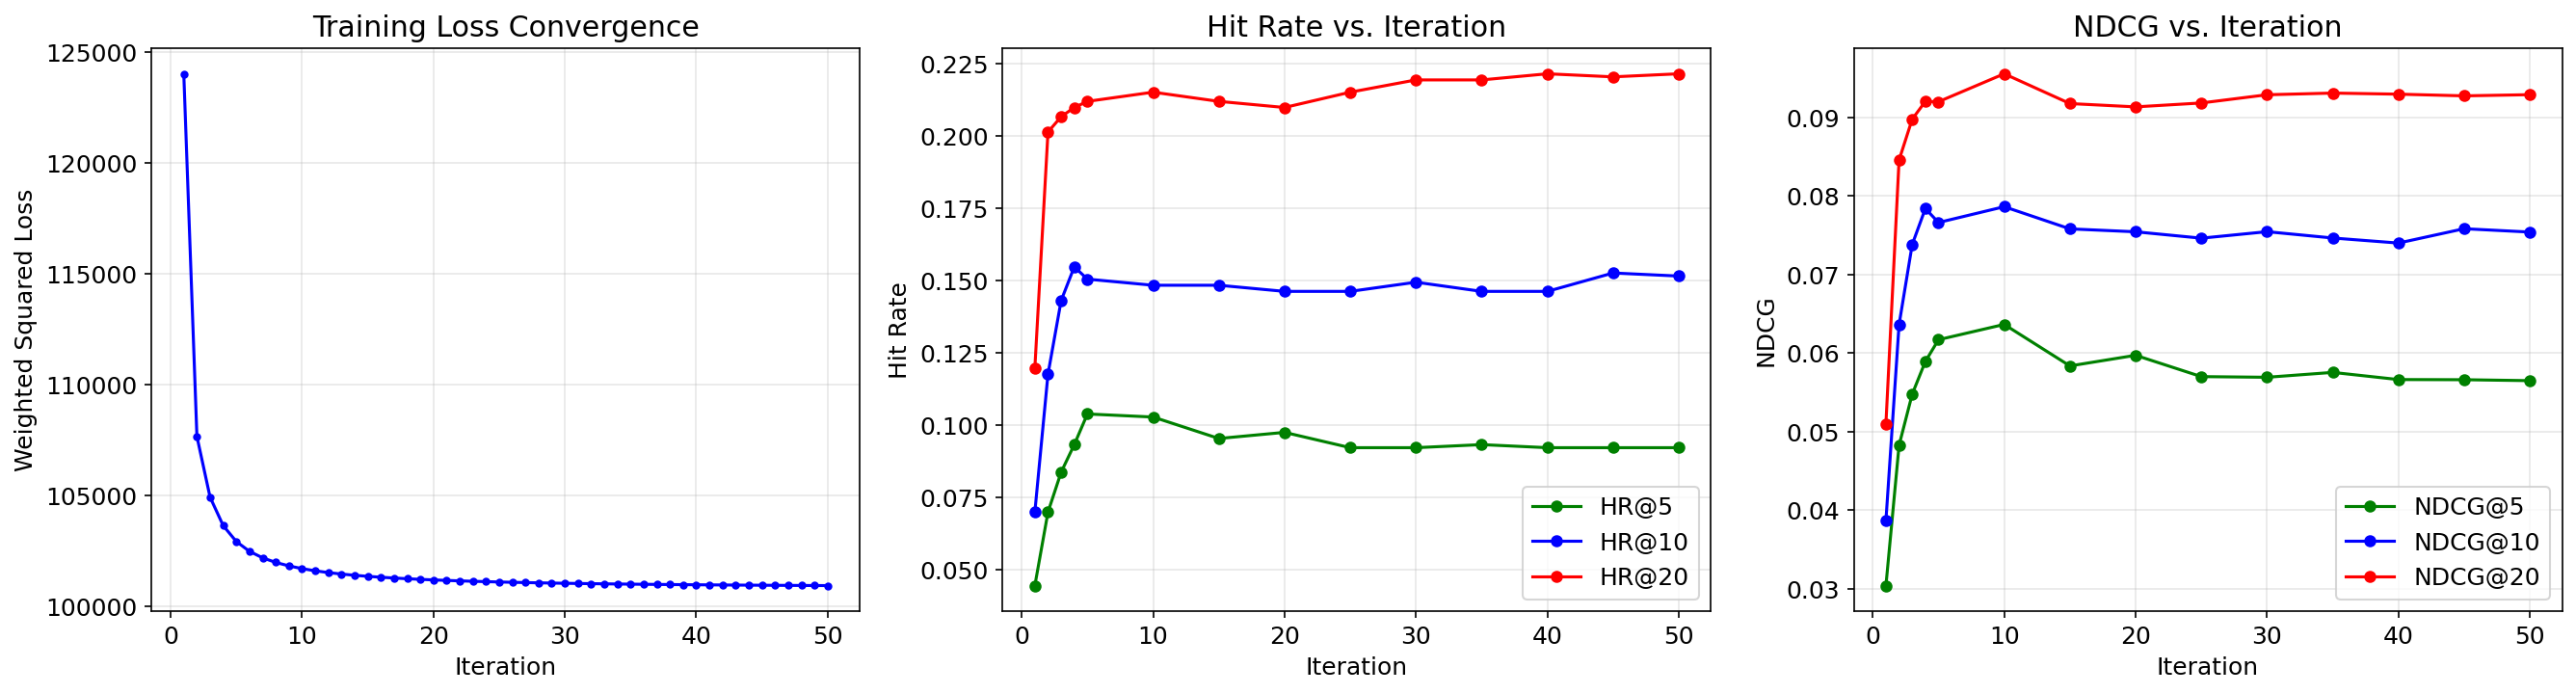
\includegraphics[width=\textwidth]{../figures/convergence.png}
\caption{Convergence over 50 iterations. Left: training loss. Center: Hit Rate at $K=5,10,20$. Right: NDCG at $K=5,10,20$.}
\label{fig:convergence}
\end{figure}

The loss (Figure~\ref{fig:convergence}, left) drops steeply during the first 5 iterations, losing roughly 20\% of its initial value, and flattens thereafter. Recommendation metrics tell a similar story: HR@10 rises from 0.070 at iteration 1 to 0.150 by iteration 5, with marginal changes after that. By iteration 20, the metrics have stabilized. Running 50 iterations produced HR@10 = 0.152, barely above the iteration-10 value of 0.148.

This confirms a known property of ALS methods: convergence is fast in the first few iterations, and additional passes yield diminishing improvements. For practical use on this dataset, 15--20 iterations would suffice.

\subsection{Effect of Latent Dimensionality}

We varied the number of latent factors $k \in \{8, 16, 32, 64\}$, training for 30 iterations each.

\begin{table}[H]
\centering
\caption{Effect of latent factors on quality and speed (30 iterations).}
\label{tab:kfactors}
\begin{tabular}{rccccr}
\toprule
$k$ & HR@5 & HR@10 & HR@20 & NDCG@10 & Avg. iter (s) \\
\midrule
8  & 0.070 & 0.121 & 0.192 & 0.056 & 0.32 \\
16 & 0.085 & 0.145 & 0.211 & 0.073 & 0.62 \\
32 & 0.092 & 0.150 & 0.220 & 0.075 & 0.84 \\
64 & 0.088 & 0.148 & 0.218 & 0.074 & 1.54 \\
\bottomrule
\end{tabular}
\end{table}

\begin{figure}[H]
\centering
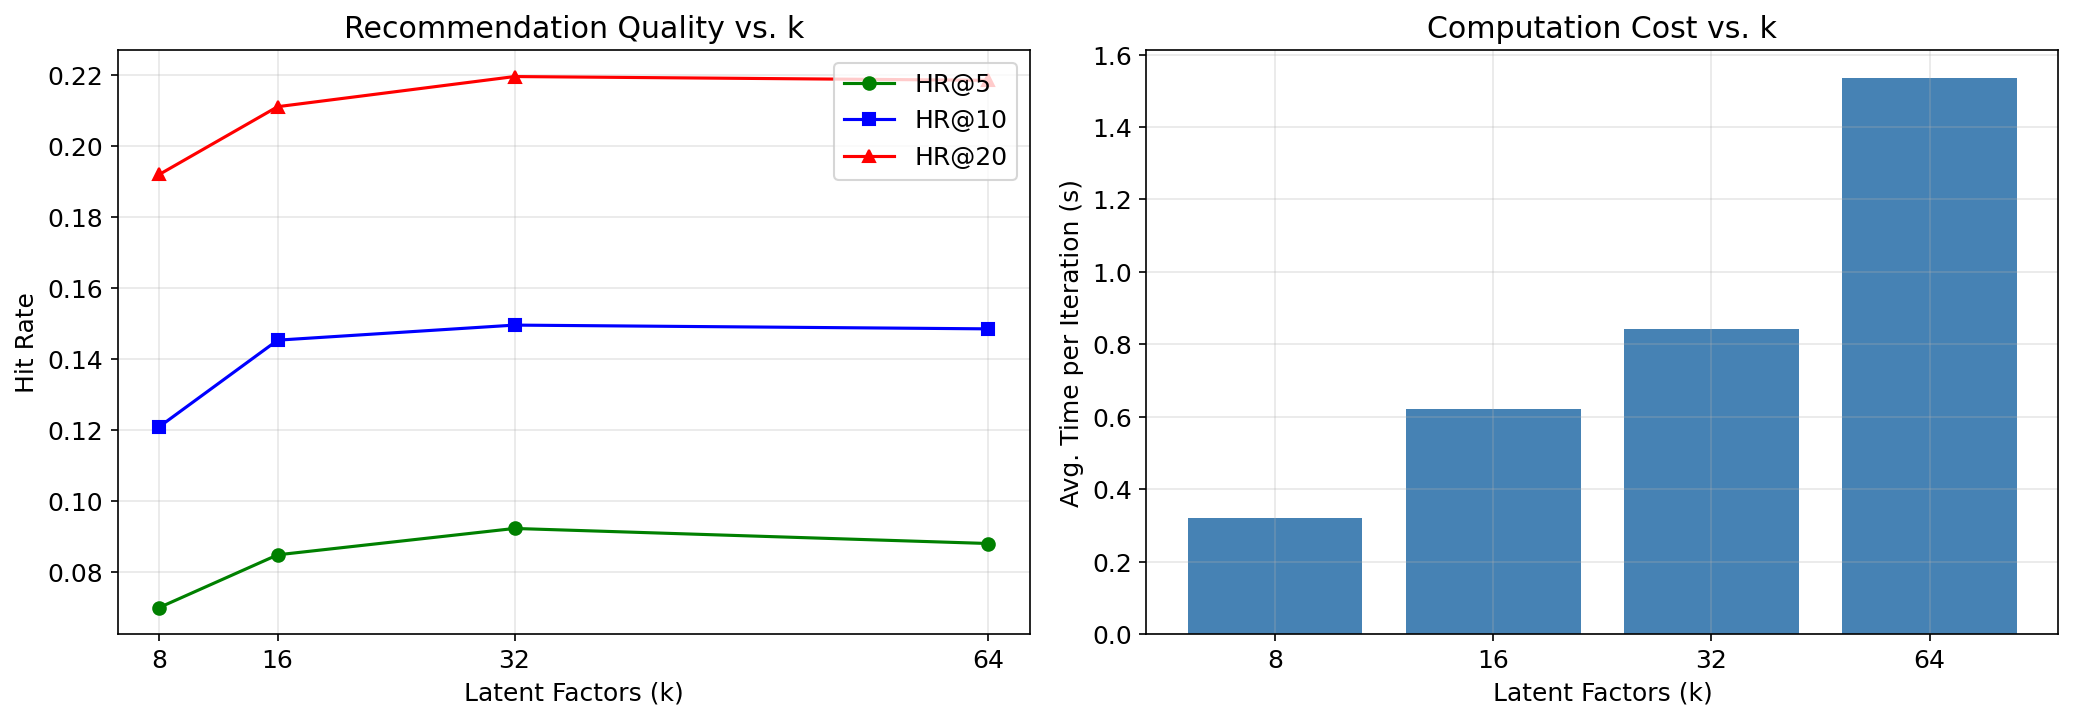
\includegraphics[width=\textwidth]{../figures/latent_factors.png}
\caption{Left: recommendation quality vs.\ $k$. Right: computation time per iteration vs.\ $k$.}
\label{fig:kfactors}
\end{figure}

Quality improves substantially from $k=8$ to $k=16$ (HR@10 jumps from 0.121 to 0.145) and more modestly from $k=16$ to $k=32$. Going to $k=64$ offers no improvement and in fact slightly degrades performance, likely due to overfitting on a dataset of this size. Meanwhile, computation time roughly doubles with each doubling of $k$, consistent with the $O(|\mathcal{R}|k + (M+N)k^2)$ complexity. For MovieLens 100K, $k=32$ gives the best quality-to-cost ratio.

\subsection{Scalability with Dataset Size}

To test how training time scales with data volume, we subsampled users at 25\%, 50\%, 75\%, and 100\%, keeping all interactions for the selected users. This varies both $M$ and $|\mathcal{R}|$ proportionally.

\begin{table}[H]
\centering
\caption{Scalability with dataset size ($k=32$, 20 iterations).}
\label{tab:scale}
\begin{tabular}{rcrrr}
\toprule
Fraction & Users & Train NNZ & Avg. iter (s) & HR@10 \\
\midrule
25\% & 235 & 24{,}762 & 0.50 & 0.128 \\
50\% & 471 & 51{,}710 & 0.62 & 0.138 \\
75\% & 707 & 76{,}027 & 0.74 & 0.149 \\
100\% & 943 & 99{,}057 & 0.81 & 0.146 \\
\bottomrule
\end{tabular}
\end{table}

\begin{figure}[H]
\centering
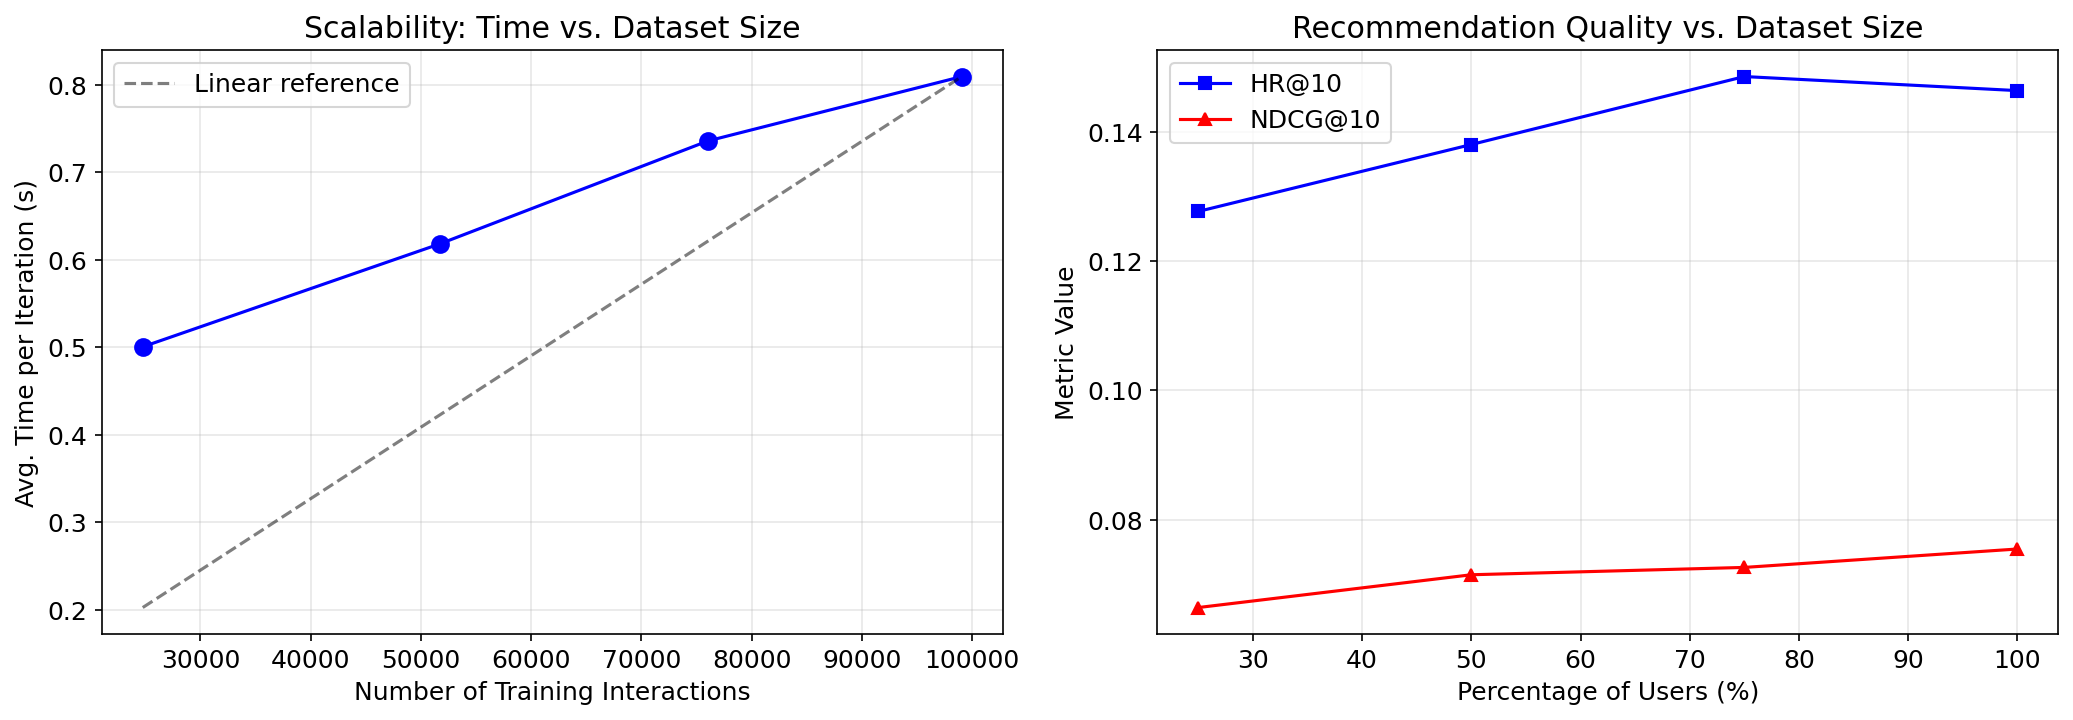
\includegraphics[width=\textwidth]{../figures/scalability.png}
\caption{Left: average iteration time vs.\ number of training interactions, with a linear reference line. Right: HR@10 and NDCG@10 vs.\ dataset fraction.}
\label{fig:scale}
\end{figure}

The time-vs-size relationship (Figure~\ref{fig:scale}, left) tracks the linear reference closely. Going from 25K to 99K interactions increased iteration time from 0.50s to 0.81s (a $1.6\times$ increase for a $4\times$ data increase). The sub-linear behavior is expected: the $O((M+N)k^2)$ term includes a fixed component from the item dimension $N$, which does not shrink proportionally when we subsample users. At larger absolute scales (millions of interactions), the $O(|\mathcal{R}|k)$ term would dominate and the scaling would approach linearity more closely.

Recommendation quality generally improves with more data (more users means more collaborative signal), though the drop at 100\% relative to 75\% is within noise for a dataset of this size.

\subsection{NumPy vs.\ PySpark RDD}

Both implementations use identical algorithms and the same random seed.

\begin{table}[H]
\centering
\caption{NumPy vs.\ Spark RDD ($k=32$, 20 iterations).}
\label{tab:impl}
\begin{tabular}{lrrrr}
\toprule
Implementation & Total (s) & Avg. iter (s) & Final loss & HR@10 \\
\midrule
NumPy & 16.35 & 0.82 & 101{,}185.6 & 0.146 \\
Spark RDD & 7.35 & 0.37 & 101{,}185.6 & 0.146 \\
\bottomrule
\end{tabular}
\end{table}

The loss sequences are identical to six decimal places across all 20 iterations (Figure~\ref{fig:spark_loss}), confirming that the Spark implementation is a faithful parallelization. The Spark version is roughly $2\times$ faster in local mode, which reflects the multi-core parallelism compensating for the serialization and JVM overhead. On a true cluster with data that doesn't fit in single-machine memory, this gap would widen in Spark's favor.

\begin{figure}[H]
\centering
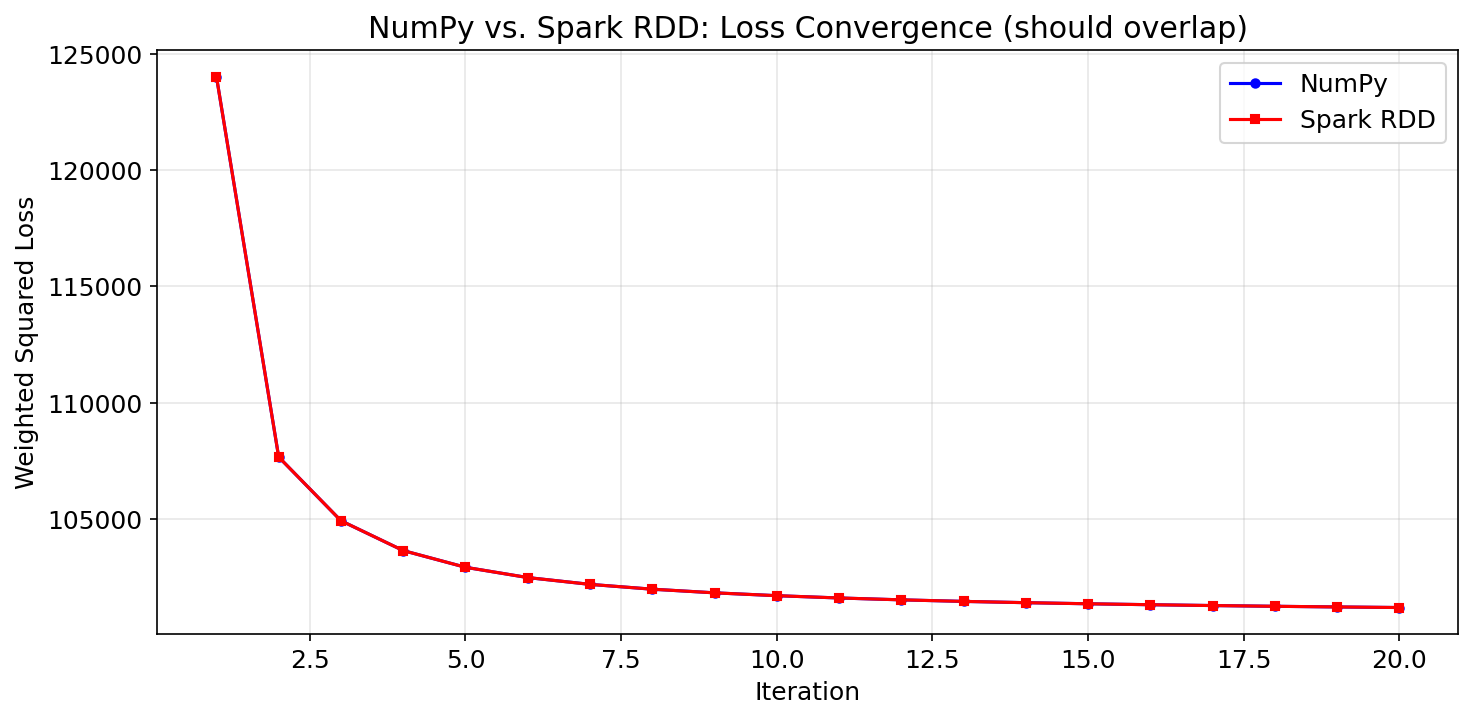
\includegraphics[width=0.7\textwidth]{../figures/numpy_vs_spark_loss.png}
\caption{Loss convergence for NumPy and Spark RDD (curves overlap exactly).}
\label{fig:spark_loss}
\end{figure}

\subsection{Comparison with Spark MLlib ALS}

We compared our eALS against Spark's built-in ALS (\texttt{pyspark.ml.recommendation.ALS}) configured for implicit feedback, with the same $k=32$ and 20 iterations.

\begin{table}[H]
\centering
\caption{eALS vs.\ Spark MLlib ALS ($k=32$, 20 iterations).}
\label{tab:baseline}
\begin{tabular}{lcccc}
\toprule
Method & HR@5 & HR@10 & HR@20 & NDCG@10 \\
\midrule
eALS (ours) & 0.092 & 0.150 & 0.220 & 0.075 \\
MLlib ALS & 0.098 & 0.154 & 0.227 & 0.079 \\
\bottomrule
\end{tabular}
\end{table}

\begin{figure}[H]
\centering
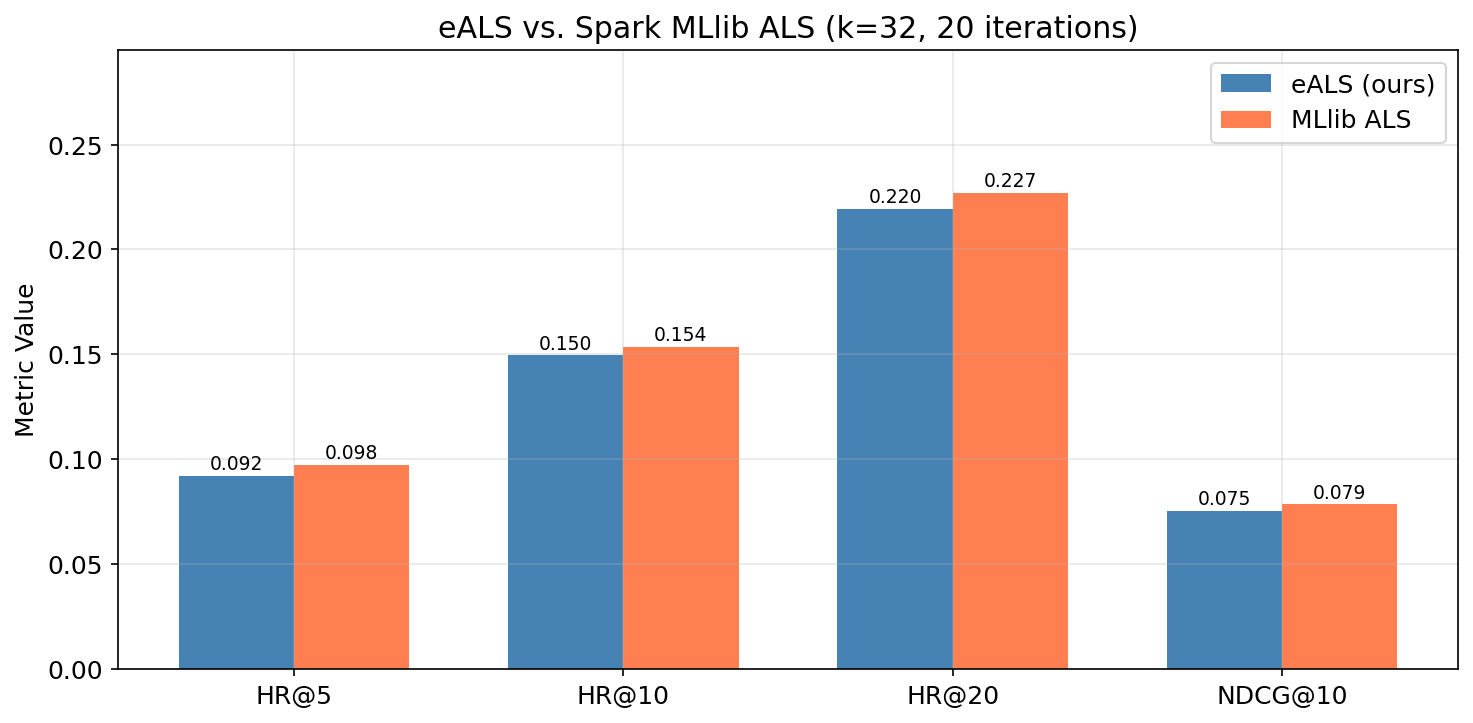
\includegraphics[width=0.7\textwidth]{../figures/eals_vs_mllib.png}
\caption{Side-by-side comparison of eALS and MLlib ALS across metrics.}
\label{fig:baseline}
\end{figure}

MLlib ALS edges out eALS by about 3\% relative on HR@10 (0.154 vs.\ 0.150). This gap is small and could be partly attributed to differences in implementation details: MLlib uses block-wise matrix partitioning and native JVM linear algebra, and its regularization and confidence weighting may differ slightly from our configuration. The two approaches are comparable in quality on this dataset.


% ============================================================
\section{Discussion: Strengths and Weaknesses}
% ============================================================

\subsection{Strengths of eALS}

\textbf{Speed per iteration.} The precomputed $\mathbf{S}^q$ matrix eliminates the need to iterate over missing entries. On MovieLens 100K, each iteration takes under a second. Standard ALS, which constructs a $k \times k$ system per user involving all $N$ items, would be roughly an order of magnitude slower.

\textbf{Straightforward parallelization.} Because user updates are independent of one another (given fixed $\mathbf{Q}$ and $\mathbf{S}^q$), distributing the work across Spark partitions required no algorithmic changes. The same element-wise update code runs on each worker; only the data shipping differs. This made the NumPy-to-Spark port mechanical rather than requiring a redesign.

\textbf{Fast convergence.} The algorithm reaches near-optimal recommendation quality within 5--10 iterations (see Section 3.1). Combined with the low per-iteration cost, total training time is practical even without distributed computing for datasets of moderate size.

\textbf{Memory efficiency.} The working set for updating a single user is the user's own $k$-vector, the $|\mathcal{I}_u| \times k$ submatrix of $\mathbf{Q}$, and the $k \times k$ matrix $\mathbf{S}^q$. For $k=32$ and a user with 100 interactions, this is about 25 KB. Workers can process users with minimal memory overhead.

\subsection{Weaknesses and Limitations}

\textbf{Driver bottleneck.} The full $\mathbf{P}$ and $\mathbf{Q}$ matrices live on the driver and are broadcast at every iteration. For MovieLens 100K this is negligible (about 400 KB for $\mathbf{Q}$ at $k=32$), but for a dataset with 10 million items the broadcast would be around 2.5 GB per half-step. At that scale, the communication cost would dominate the computation.

\textbf{Sequential factor updates within a user.} The element-wise update processes factors $f=0,1,\ldots,k-1$ sequentially because each update depends on the prediction cache, which is modified by the previous update. This inner loop cannot be parallelized. For large $k$, this serial dependency becomes the tightest bottleneck.

\textbf{Uniform weighting of missing data.} Our implementation uses a single weight $c_0$ for all missing entries. The paper also proposes item-popularity-based weighting (items interacted with by more users get higher missing-data weight), which can improve quality. We did not implement this variant due to time constraints.

\textbf{Limited dataset scale.} MovieLens 100K is small enough that single-machine NumPy is already fast ($\sim$0.8s per iteration). The benefit of Spark parallelization is modest at this scale ($2\times$ on a multi-core laptop). A proper scalability study would require MovieLens 10M or a larger dataset to show where the distributed version becomes necessary rather than optional. We were limited by the available compute environment.

\textbf{No online update evaluation.} The paper's title references ``online recommendation,'' and eALS supports incremental updates when new interactions arrive (by updating only the affected user/item vectors without retraining from scratch). We implemented only the batch training and did not test incremental updates.

\subsection{Comparison with MLlib}

MLlib ALS slightly outperformed our eALS on all metrics (Table~\ref{tab:baseline}). Two factors likely explain this. First, MLlib's implementation is heavily optimized at the JVM level with native BLAS calls, while our element-wise updates run in Python loops. Second, MLlib uses a different ALS formulation (standard block-wise) that solves the full $k$-dimensional system per user, which may converge to a slightly better optimum for the same number of iterations. The gap is small enough (3\% relative) that it does not diminish the practical value of eALS, particularly given its lower per-iteration computational cost.


% ============================================================
\section*{References}
% ============================================================

\begin{thebibliography}{9}
\bibitem{he2016}
X.~He, H.~Zhang, M.-Y.~Kan, and T.-S.~Chua.
\textit{Fast Matrix Factorization for Online Recommendation with Implicit Feedback}.
In Proceedings of SIGIR, 2016.

\bibitem{hu2008}
Y.~Hu, Y.~Koren, and C.~Volinsky.
\textit{Collaborative Filtering for Implicit Feedback Datasets}.
In Proceedings of IEEE ICDM, 2008.
\end{thebibliography}


% ============================================================
\appendix
\section{Full Source Code}
\label{sec:code}
% ============================================================

\subsection{data\_loader.py}
\lstinputlisting[language=Python]{../src/data_loader.py}

\subsection{eals\_numpy.py}
\lstinputlisting[language=Python]{../src/eals_numpy.py}

\subsection{eals\_rdd.py}
\lstinputlisting[language=Python]{../src/eals_rdd.py}

\subsection{evaluation.py}
\lstinputlisting[language=Python]{../src/evaluation.py}


\end{document}
